%%%%%%%%%%%%%%%%%%%%%%%%%%%%%%%%%%%%%%%%%%%%%%%%%%%%%%%%%%%%%%%%%%%%%
% PREAMBLE
%%%%%%%%%%%%%%%%%%%%%%%%%%%%%%%%%%%%%%%%%%%%%%%%%%%%%%%%%%%%%%%%%%%%%

%% Start with one of the following:
% DOUBLE-SPACED VERSION FOR SUBMISSION TO THE AMS
\documentclass{ametsoc}

% TWO-COLUMN JOURNAL PAGE LAYOUT---FOR AUTHOR USE ONLY
% \documentclass[twocol]{ametsoc}

%%%%%%%%%%%%%%%%%%%%%%%%%%%%%%%%
%%% To be entered only if twocol option is used

\journal{jpo}

%  Please choose a journal abbreviation to use above from the following list:
% 
%   jamc     (Journal of Applied Meteorology and Climatology)
%   jtech     (Journal of Atmospheric and Oceanic Technology)
%   jhm      (Journal of Hydrometeorology)
%   jpo     (Journal of Physical Oceanography)
%   jas      (Journal of Atmospheric Sciences)	
%   jcli      (Journal of Climate)
%   mwr      (Monthly Weather Review)
%   wcas      (Weather, Climate, and Society)
%   waf       (Weather and Forecasting)
%   bams (Bulletin of the American Meteorological Society)
%   ei    (Earth Interactions)

%%%%%%%%%%%%%%%%%%%%%%%%%%%%%%%%
%Citations should be of the form ``author year''  not ``author, year''
\bibpunct{(}{)}{;}{a}{}{,}

%%%%%%%%%%%%%%%%%%%%%%%%%%%%%%%%

%%% To be entered by author:

%% May use \\ to break lines in title:

\title{Barotropic vorticity balance of the North Atlantic subpolar gyre in a strongly eddying model}

%%% Enter authors' names, as you see in this example:
%%% Use \correspondingauthor{} and \thanks{Current Affiliation:...}
%%% immediately following the appropriate author.
%%%
%%% Note that the \correspondingauthor{} command is NECESSARY.
%%% The \thanks{} commands are OPTIONAL.

    %\authors{Author One\correspondingauthor{Author One, 
    % American Meteorological Society, 
    % 45 Beacon St., Boston, MA 02108.}
% and Author Two\thanks{Current affiliation: American Meteorological Society, 
    % 45 Beacon St., Boston, MA 02108.}}

\authors{M. Lecorre\correspondingauthor{Laboratoire d’Oc\'eanographie Physique et Spatiale (LOPS), IUEM, Brest, France.}, J. Gula, and A.-M. Tr\'eguier}

%% Follow this form:
    % \affiliation{American Meteorological Society, 
    % Boston, Massachusetts.}

\affiliation{Univ. Brest, CNRS, IRD, Ifremer, Laboratoire d’Océanographie Physique et Spatiale (LOPS), IUEM, Brest, France}

%% Follow this form:
    %\email{latex@ametsoc.org}

\email{mathieu.lecorre@univ-brest.fr}

%% If appropriate, add additional authors, different affiliations:
    %\extraauthor{Extra Author}
    %\extraaffil{Affiliation, City, State/Province, Country}

  
%\extraauthor{}
%\extraaffil{}

%% May repeat for a additional authors/affiliations:

%\extraauthor{}
%\extraaffil{}

%%%%%%%%%%%%%%%%%%%%%%%%%%%%%%%%%%%%%%%%%%%%%%%%%%%%%%%%%%%%%%%%%%%%%
% ABSTRACT
%
% Enter your abstract here
% Abstracts should not exceed 250 words in length!
%
% For BAMS authors only: If your article requires a Capsule Summary, please place the capsule text at the end of your abstract
% and identify it as the capsule. Example: This is the end of the abstract. (Capsule Summary) This is the capsule summary. 

\abstract{hihi}

\begin{document}


\section{Model and set-up}
%\subsection{Model setting}


%To investigate the impact of the topography on the circulation, it is essential to have a good representation of the flow-topography interaction. To do so, we use a terrain-following coordinate model: the Regional Oceanic Modelling System (ROMS, \citet{shchepetkin2009}) in its CROCO (Coastal and Regional Ocean Community) version \citep{debreu2012}. It solves the hydrostatic primitive equation for velocity, temperature and salinity, using a full equation of state for seawater \citep{shchepetkin2009,shchepetkin2011}. The North Atlantic domain has 1450 $\times$ 1300 points  with a horizontal resolution of 5--6 km. The simulation is eddy permitting in most of the area, as the Rossby deformation radius varies between 10 and 20 km over the region \citep{chelton1998}. The domains are shown in figure \ref{domain}. 

%Bathymetry the domain is constructed from the SRTM30 PLUS dataset (available online at \url{http://topex.ucsd.edu/WWW_html/srtm30_plus.html}) based on the 1 min \citep{sandwell1997} global dataset and higher resolution data where available. A Gaussian smoothing kernel with a width 4 times the topographic grid spacing is used to avoid aliasing whenever the topographic data are available at higher resolution than the computational grid and to ensure the smoothness of the topography at the grid scale. Also, to avoid pressure gradient errors induced by terrain-following coordinates in shallow regions with steep bathymetric slope \citep{beckmann1993}, we apply local smoothing of the bottom topography where the steepness of the topography exceeds a factor r=0.2. 

%Initial and horizontal boundary data are taken from the Simple Ocean Data Assimilation (SODA, \citet{carton2008}). The simulation is run from January 1st, 2000 to December 31st, 2010. It is spun up for 3 years. The surface forcings are daily ERA-INTERIM data for the parent grid. A weak salinity correction flux is used at the surface of the domain toward the ISAS13 climatology \citep{gaillard2016} to account for missing freshwater fluxes in the western part of the domain.

%The North Atlantic simulation has 50 vertical levels. Vertical levels are stretched at the surface and bottom \citep{lemarie2012} to have a better representation of the surface layer dynamics at the top and flow-topography interactions at the bottom. The depth of the transition between flat z levels and terrain-following $\sigma$ levels is $h_{cline} = 300$ m. The two parameters controlling the bottom and surface refinement of the grid are $\sigma _b=2$, $\sigma _s=7$. The vertical mixing of tracers and momentum is done by a k-$\epsilon$ model (GLS, \citet{umlauf2003}). The effect of bottom friction is parameterized through a logarithmic law of the wall with a roughness length $Z_{0} = 0.01$ m.

%\begin{figure}[t]
%\centerline{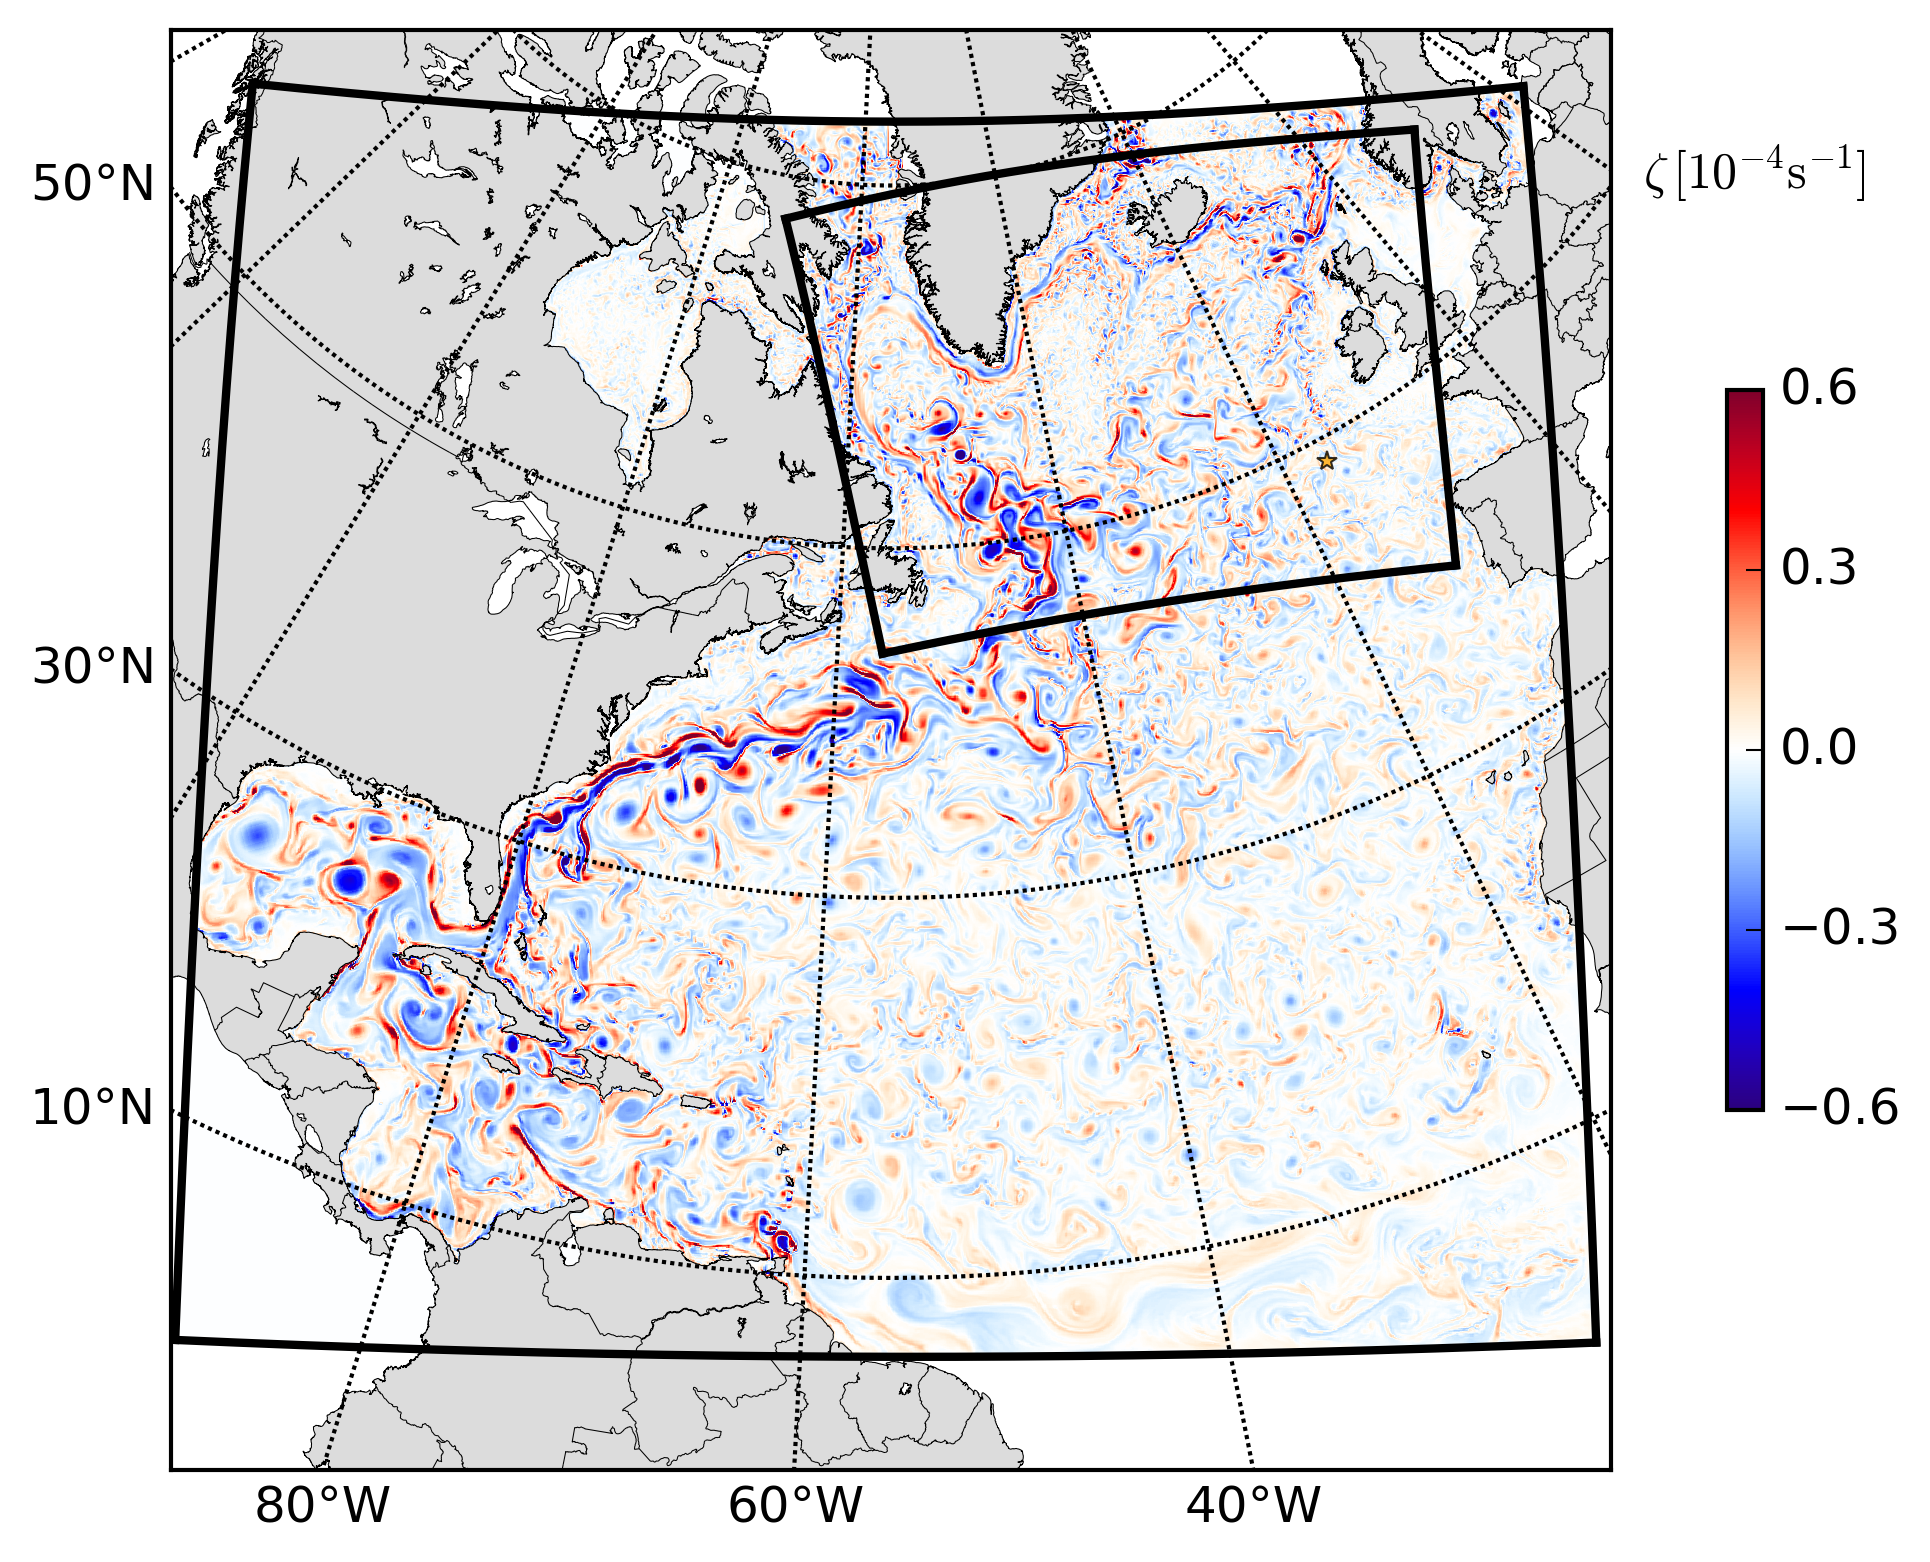
\includegraphics[width=15cm]{./fig/vrt500_and_nest.png}}
%\caption{Snapshot of the relative vorticity at 500 m depth in the Noth Atlantic. The parent grid ($\Delta x \approx 6$ km) covers most the North atlantic, and the child grid ($\Delta x \approx 2$ km) covers the subpolar gyre.}
%\label{domain}

%\end{figure}



\begin{figure}[H]
\centerline{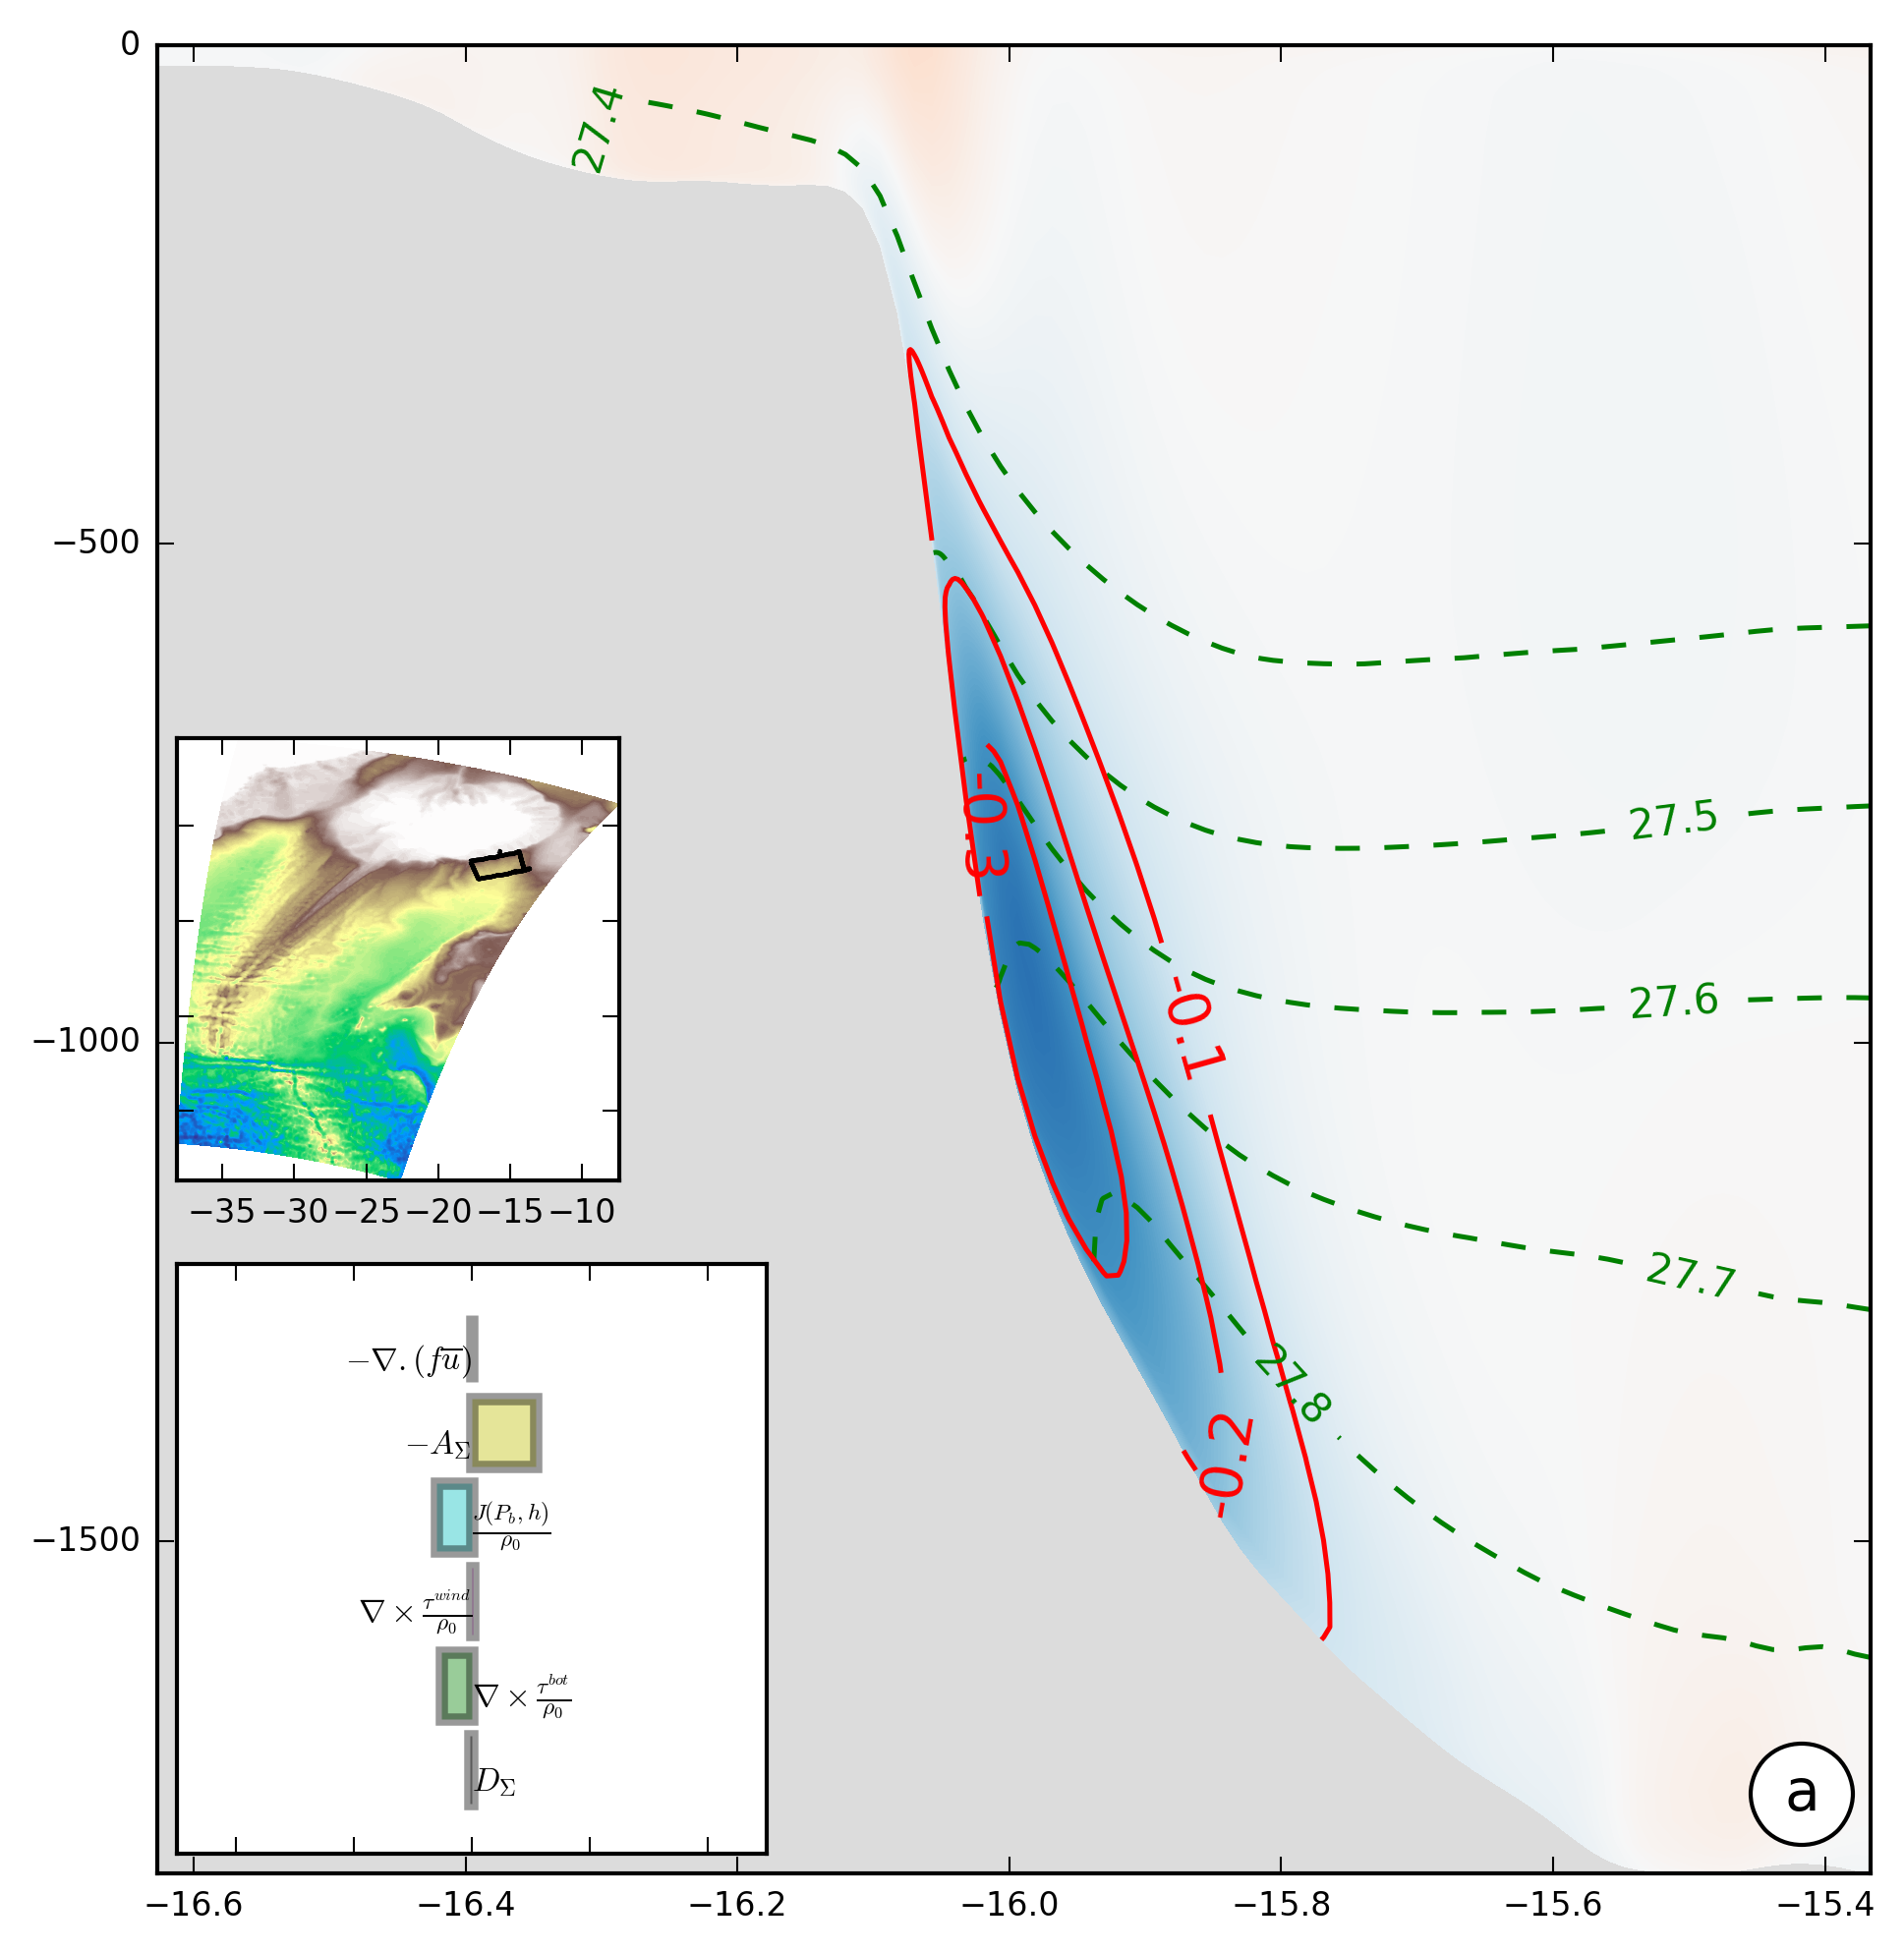
\includegraphics[width=7cm]{./v_b/section_RR_1.png}
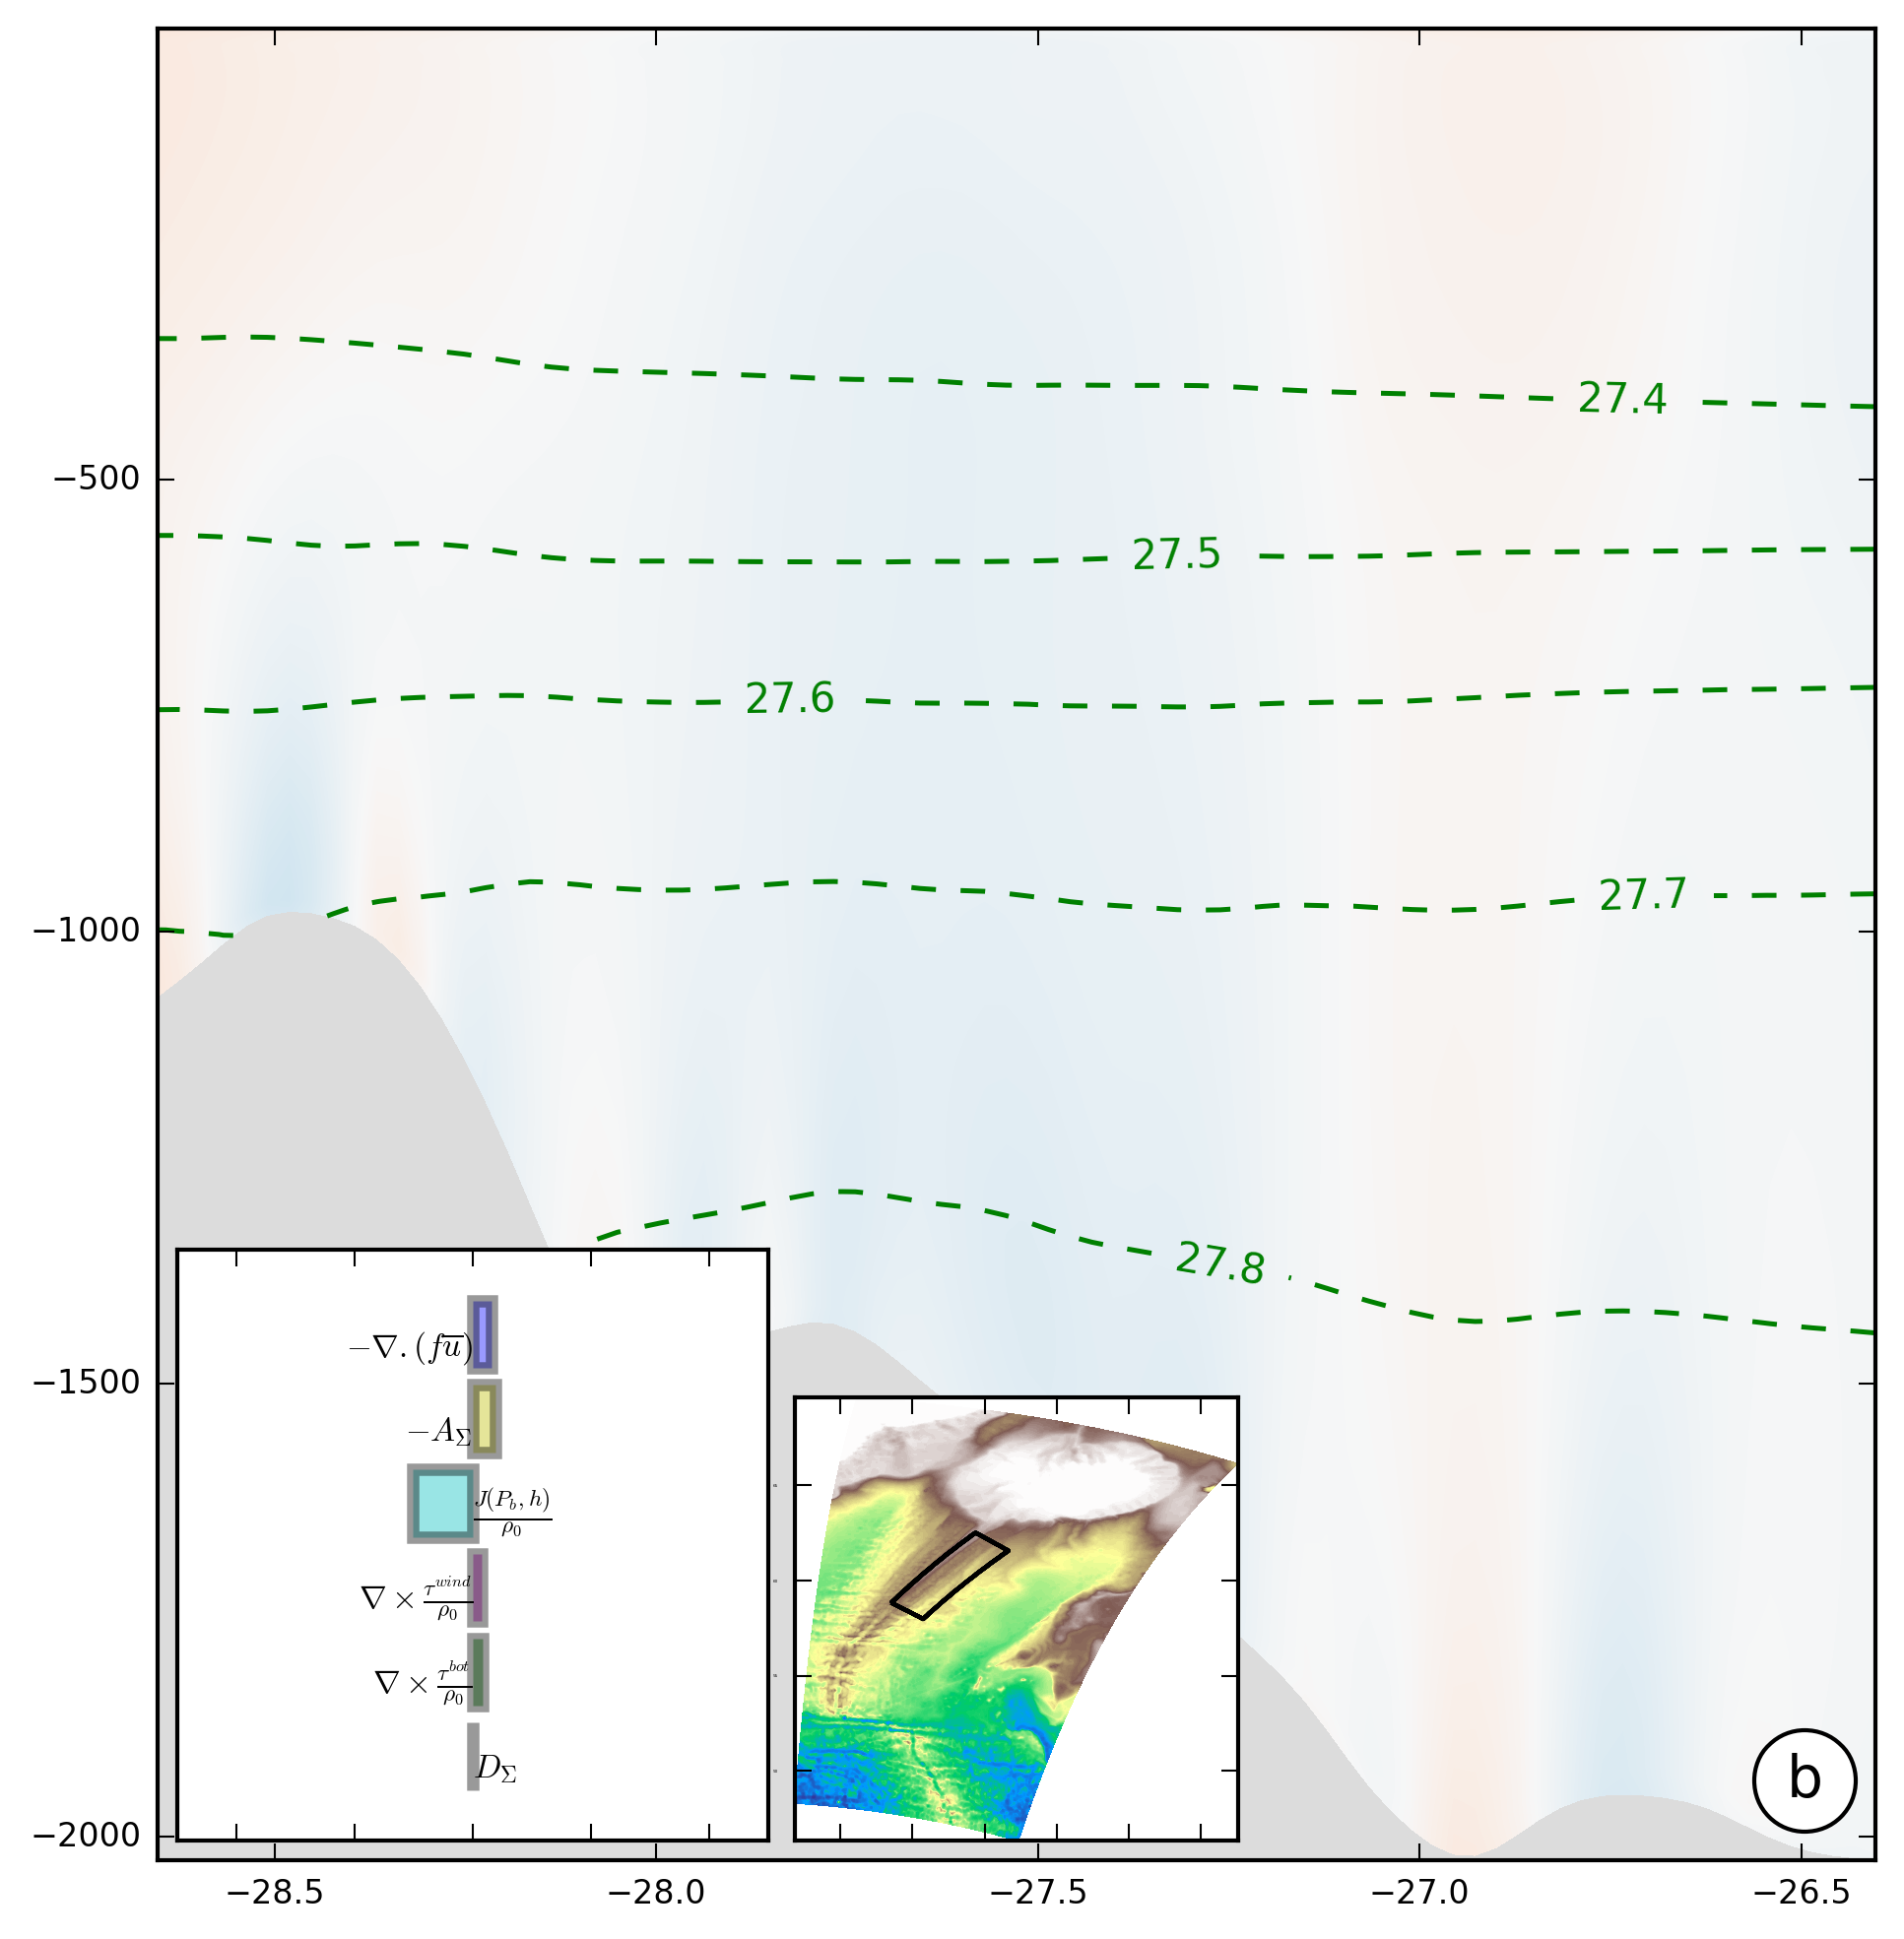
\includegraphics[width=7cm]{./v_b/section_RR_2.png}}
\centerline{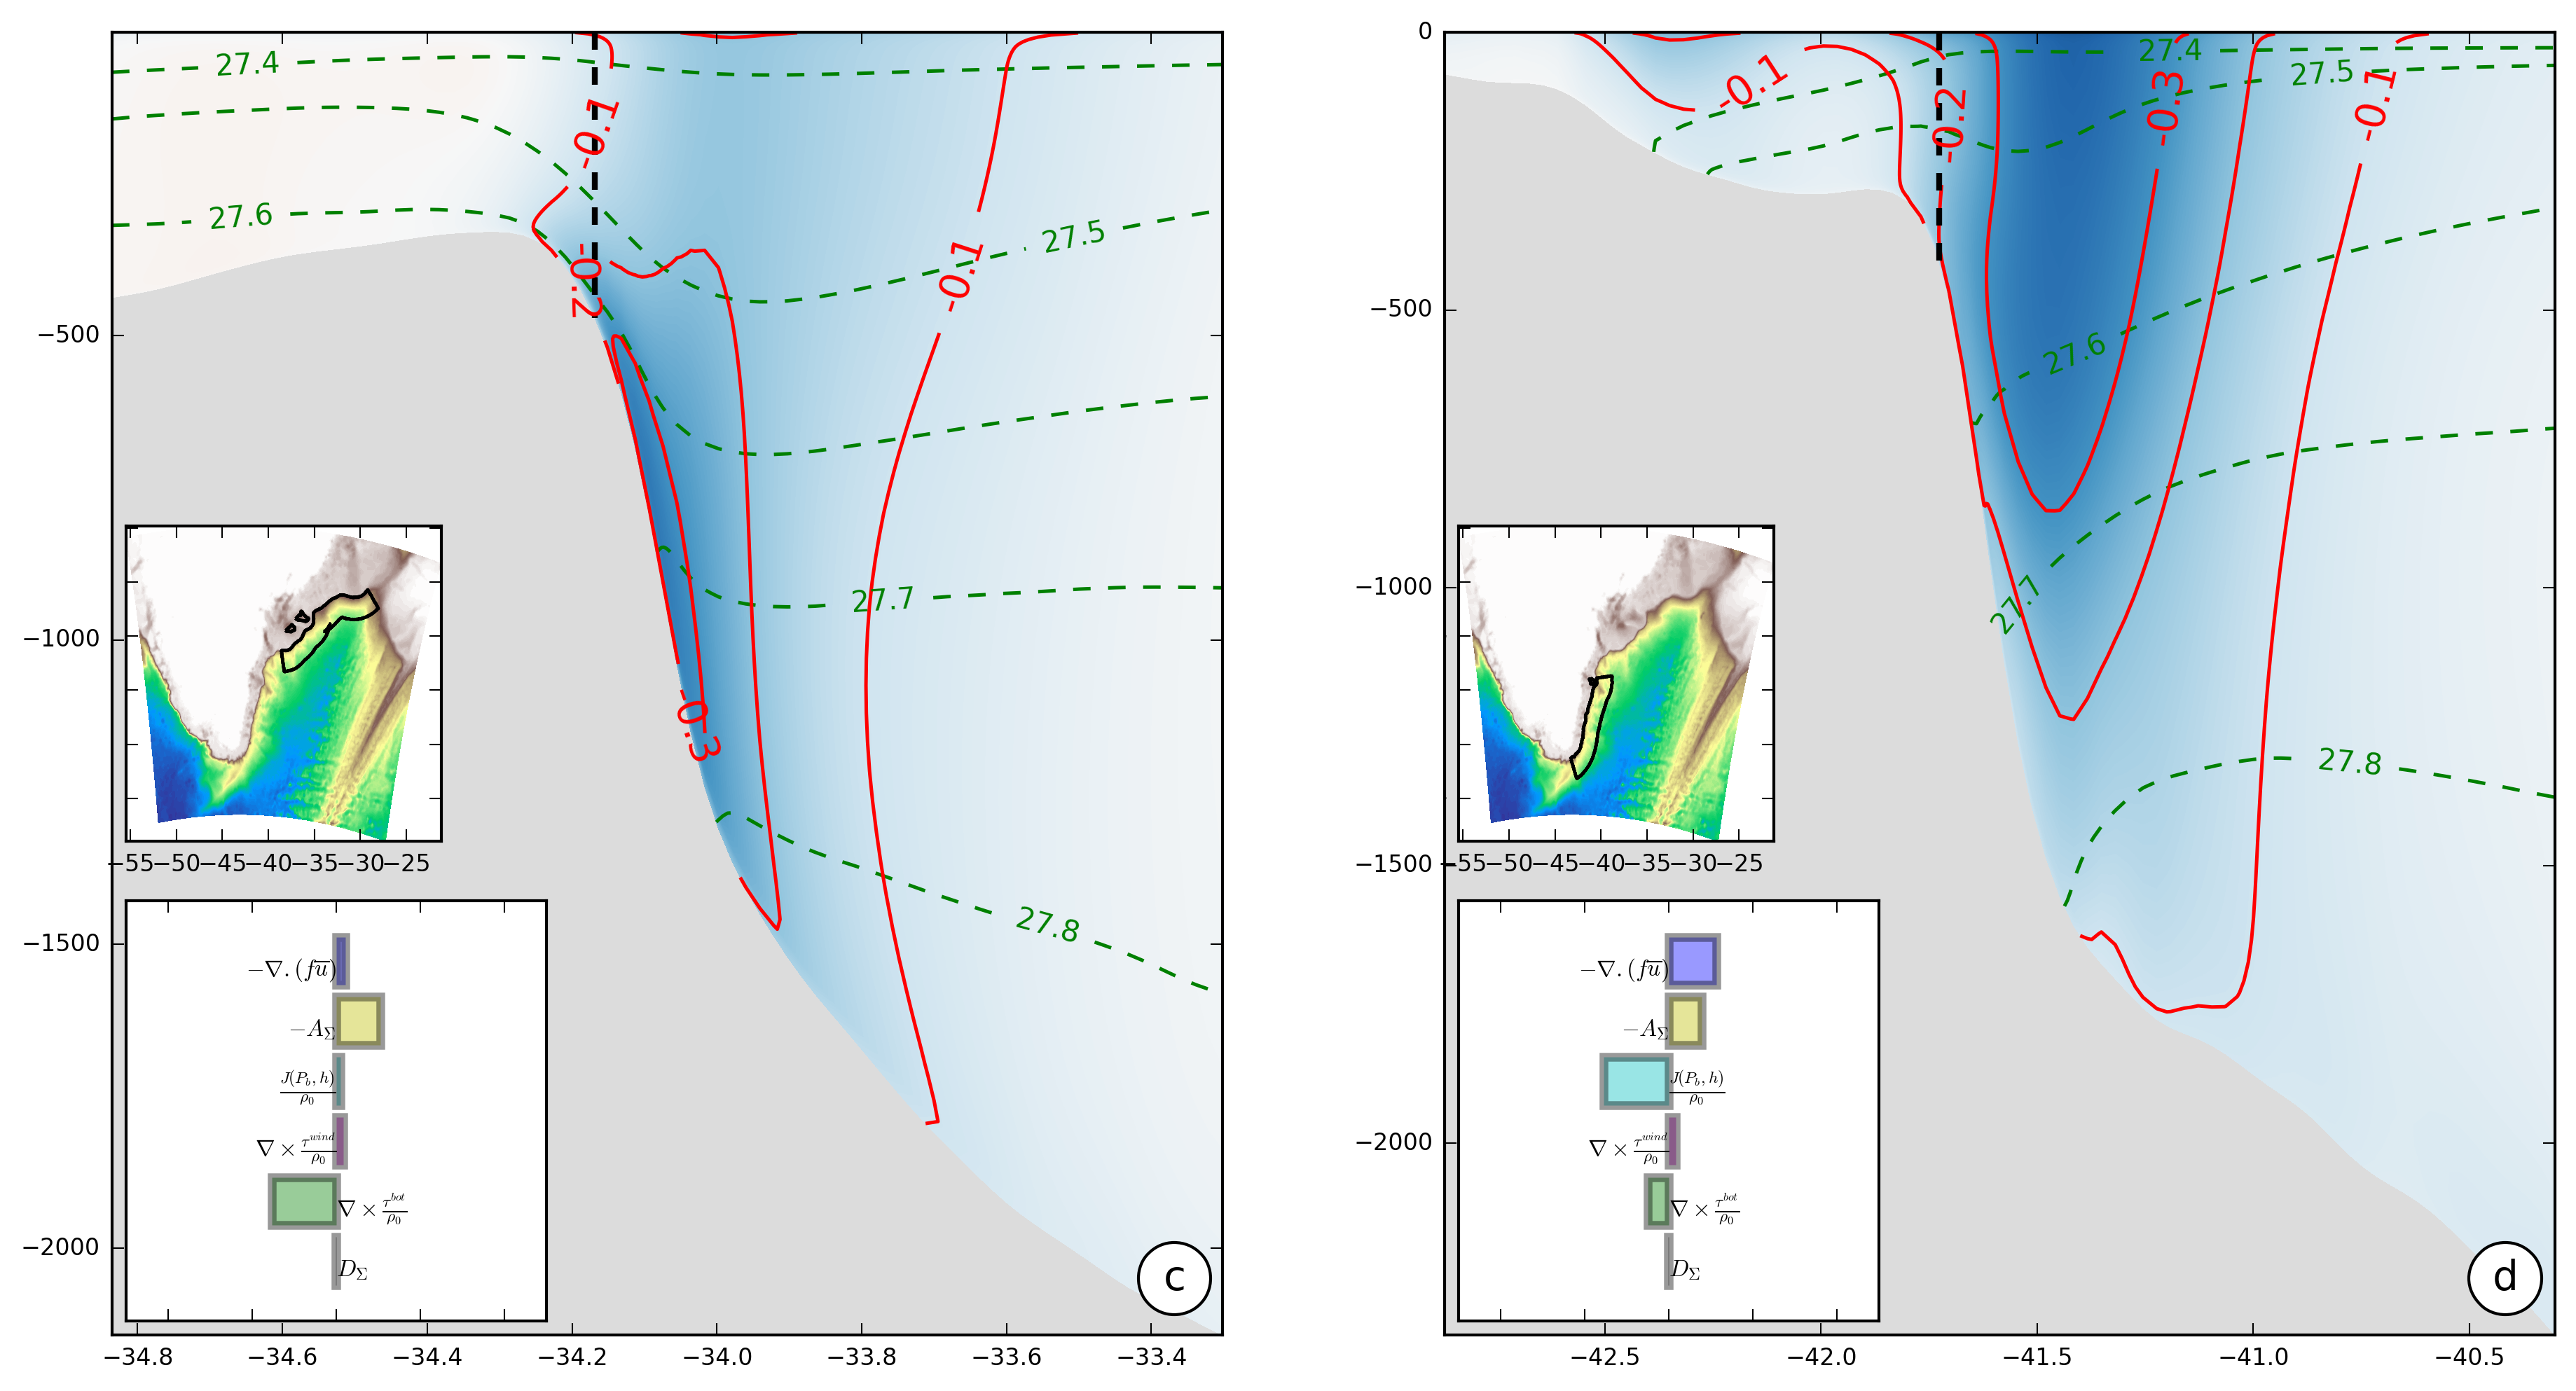
\includegraphics[width=14cm]{./v_b/section_green.png}}
\centerline{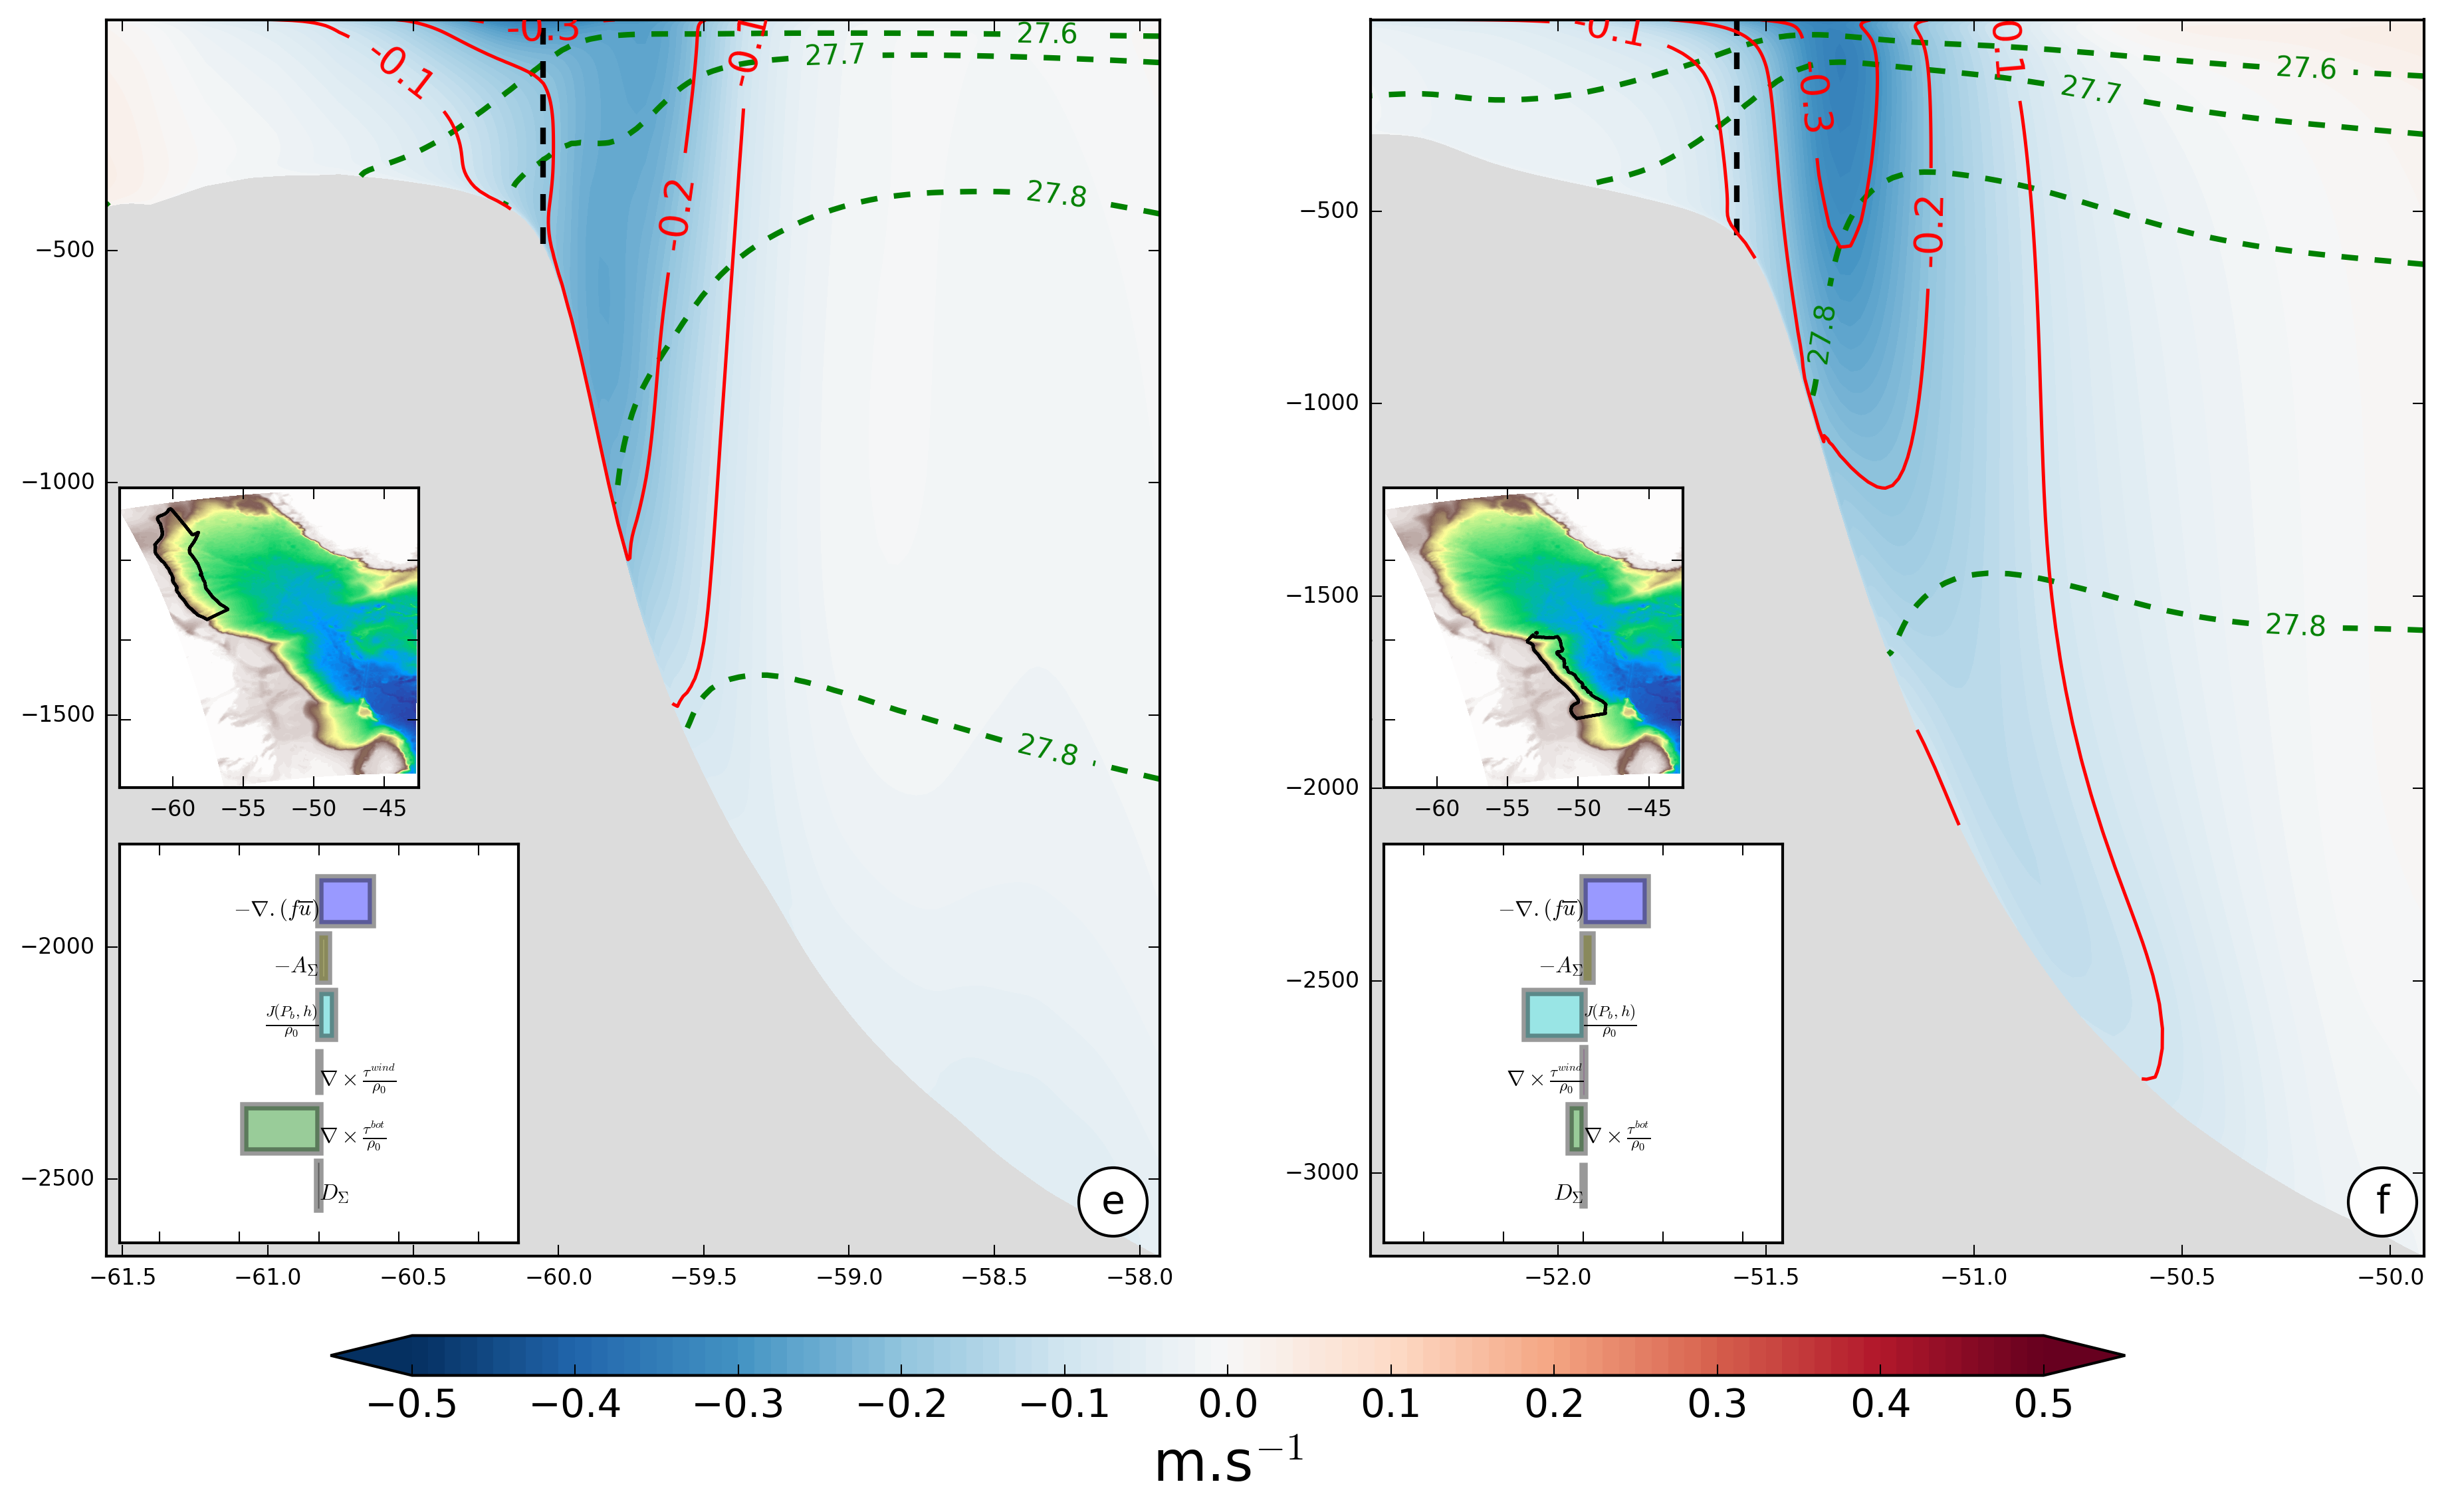
\includegraphics[width=14cm]{./v_b/section_lab.png}}
\label{int_NL}
\end{figure} 

%We divide our boundary part in six subsections. Each subsection are corresponding to change in the main direction of the flow (Northward,Southward) which creates the following decomposition (from East to West): Iceland Basin (IC) ,Eastern RR (ERR), Western RR (WRR), Eastern Greenland (EG), Western Greenland (WG) and Western Labrador Sea (WLS). The Barotropic Vorticity Balance integrated on the areas shows several specific dynamics of BC.

%When $-\nabla.(f\overline{u}<0$) (Northward flow, in cyan in figure. \ref{bv_zones}) the dynamics is linked to an equilibrium between BPT and the NL term (IB, WRR, WG). High value of NL term can be related to eddy generation near the topograpgy (see EKE and EAPE map). As these areas have eddy activity, non linear term is increased which is compensated by an increase of BPT with vertical steering (variation of the ssh) and isopycnal displacements. 

%On ERR (in blue figure. \ref{bv_zones}) in the planetary vorticity is close to zero as all the water is zonally crossing the ridge and does not recirculate back into the Iceland Basin. The equilibrium is done between the BPT, the wind and NL term. The presence of the NL term allows the flow to cross the f/h contour increasing the cross ridge transport.

%For areas around Greenland and along the Canadian coastline, we do not take into account the outter part of the jet corresponding to interaction's zone with the shelf, where thedynamics is separated from the open ocean. Be aware that the results are only represented inner part of the jet. A complete view of the jet would imply a smaller amplitude values for BPT and BDC as the equilibrium on the shelf is mainly between those two components.

%In the WLS the main contributors of positive BV are the planetary vorticity and the BPT and are being compensated by the BDC and NL term. In fact we have two regime along the WLS explaining why the equilibrium is different from what we usually have. Those two regimes can be separeted by the 57.5$^{\circ}$N latitude line. On the Southern part of the domain we retrieve the usual balance between the $\beta$-effect and the BPT with a strong BDC signal. Northern of this we have a positive $-\beta$V signal meaning a negative meridional velocity, along with this the topography is "going away" from the meridional direction. It means that the flow is going down isobath. To balance this a positive signal of BPT is needed to callback the flow to isobath. The positive input of vorticity is balanced by a strong signal of bottom BDC and NL term. Then the small amplitude of BPT can be explain as we have two regions with a change of sign while other term do not change sign explaining there high amplitudes. 

%The same equilibirum appears on EG. On the northern part, south of the Danemark Strait, BPT and $-\beta$V have the same sign which explain the strong signal of BDC. On the Southern part, even if the topography is "going away" from the meridional direction the BPT and $\beta$-efect have opposite sign. This is due to a strong wind signal forcing the flow to go up topography. 

%l'idée est la suivante, compte tenu du fait que l'équilibre près de la topographie correspond à un équilibre entre BV et BPT, si la vitesse méridonnal tend à faire monter les masses d'eaux sur la topography, le BPT va agir pour faire suivre une isobath au courant en le faisant "redescendre" ce qui correspond à une valeur négative. En calculant donc l'angle entre la "direction" de la topographie et le vecteur vitesse méridionnal on peut avoir un avant gout du signe du BPT. 
%Ex:
%-Si V est négatif (-BV positif) et si angle négatif, la topo "fuit" le vecteur V, le BPT va devoir faire "remonter" le courant et donc être positif.
%-Si V est négatif (-BV positif) et si angle positif, la topo "rencontre" le vecteur V, le BPT va devoir faire "descendre" le courant et donc être négatif.
%-Si V est positif (-BV négatif) et si angle positif, la topo "fuit" le vecteur V, le BPT va devoir faire "remonter" le courant et donc être positif.
%-Si V est positif (-BV négatif) et si angle négatif, la topo "rencontre" le vecteur V, le BPT va devoir faire "descendre" le courant et donc être négatif.

\bibliographystyle{ametsoc2014}
\bibliography{vort_240419}

%\centerline{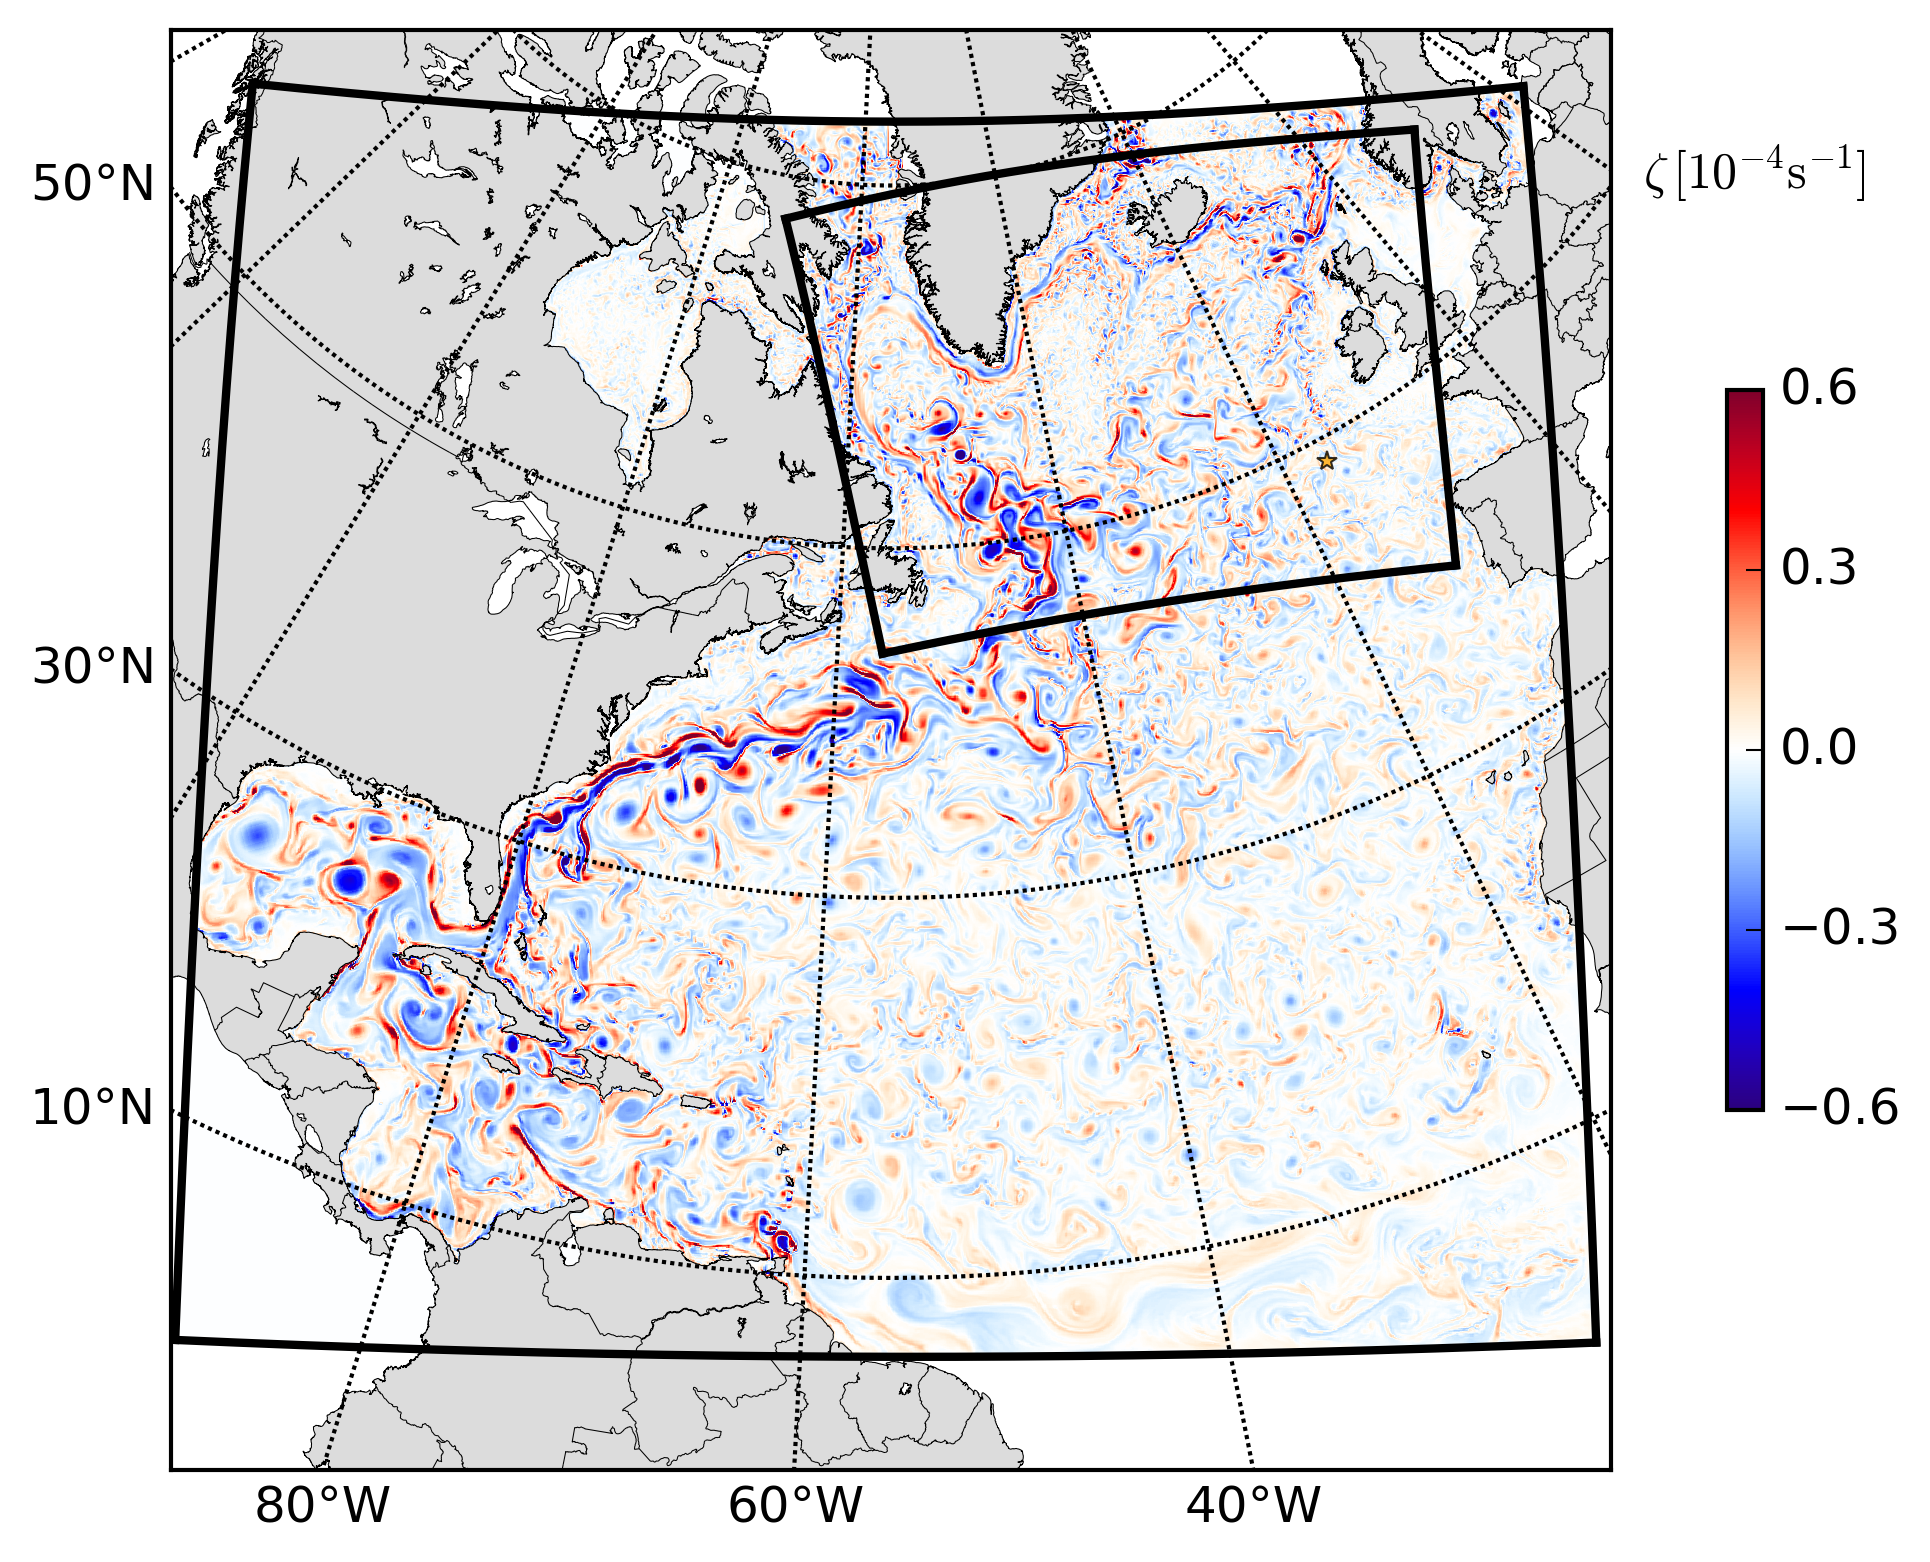
\includegraphics[width=15cm]{./fig/vrt500_and_nest.png}}
%\caption{Snapshot of the relative vorticity at 500 m depth in the Noth Atlantic. The parent grid ($\Delta x \approx 6$ km) covers most the North atlantic, and the child grid ($\Delta x \approx 2$ km) covers the subpolar gyre.}
%\label{domain}

%\centerline{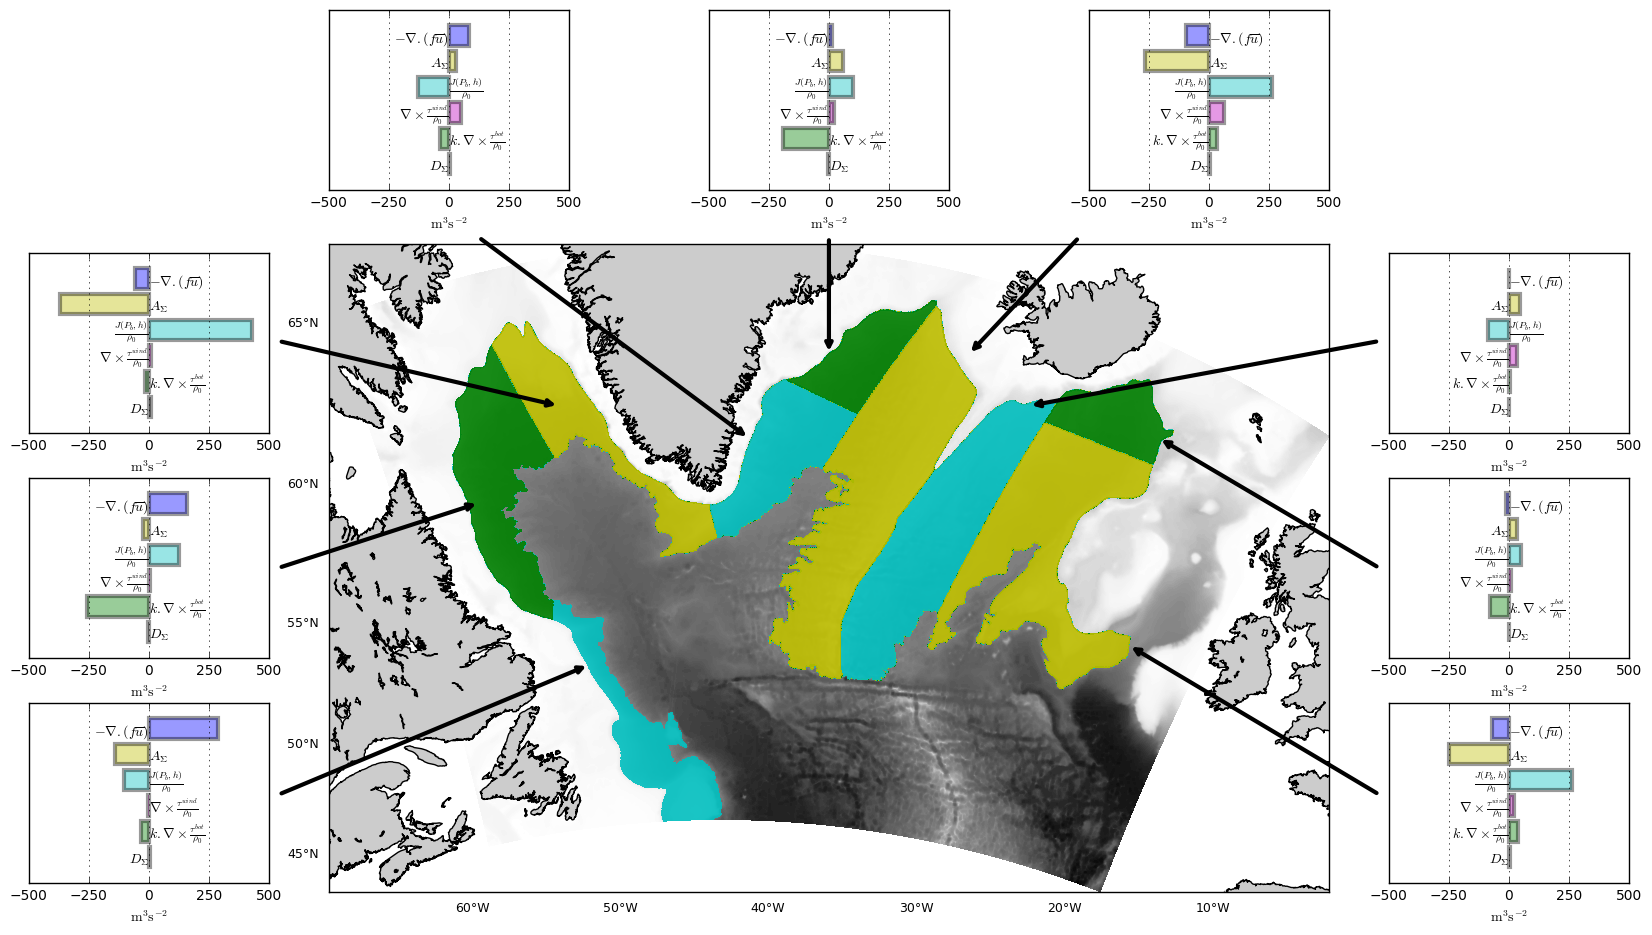
\includegraphics[width=15cm]{./v_b/int_sous_zones_3sv.png}}
%\caption{Barotropic vorticity balance integrated on different parts of the gyre near the topography}
%\label{bv_zones}
%\end{figure}

\end{document}